\documentclass[12pt,a4paper]{report}

% ---------- packages ----------
\usepackage[T1]{fontenc}
\usepackage[utf8]{inputenc}
\usepackage{lmodern}
\usepackage{microtype}
\usepackage[top=2.5cm, bottom=2.5cm, left=3cm, right=2.5cm]{geometry}
\usepackage{graphicx}
\usepackage[hidelinks]{hyperref}
\usepackage{fancyvrb}
\usepackage{xcolor}
\definecolor{codegray}{rgb}{0.95,0.95,0.95}
\usepackage{booktabs}
\usepackage{float}
\usepackage{parskip}
\usepackage{fancyhdr}
\usepackage{titlesec}
\usepackage{array}
\usepackage{longtable}
\usepackage{enumitem}
\usepackage{caption}
\usepackage{subcaption}
\usepackage{pdfpages}
\usepackage{textcomp}

% ---------- headers / footers ----------
\pagestyle{fancy}
\fancyhf{}
\fancyhead[L]{\small\leftmark}
\fancyhead[R]{\small Internet Banking System}
\fancyfoot[C]{\thepage}
\renewcommand{\headrulewidth}{0.4pt}

% ---------- chapter title style ----------
\titleformat{\chapter}[display]
  {\normalfont\huge\bfseries}
  {\chaptertitlename\ \thechapter}{20pt}{\Huge}

% ---------- document ----------
\begin{document}

% =========================================================
% TITLE PAGE
% =========================================================
\begin{titlepage}
  \centering
  \vspace*{2cm}
  {\Large\scshape Silesian University of Technology \par}
  \vspace{3cm}
  \rule{\linewidth}{0.5mm}\\[0.4cm]
  {\huge\bfseries Internet Banking System\par}
  \vspace{0.3cm}
  {\Large Technical Project Report\par}
  \rule{\linewidth}{0.5mm}\\[1.5cm]

  \begin{tabular}{l}
    Piotr Krupi\'nski \\[0.8em]
    Jeremi Szczotka \\[0.8em]
    Szymon Ma\'nka \\[0.8em]
    Hyunseok Cho \\[0.8em]
    Sim\~ao Galv\~ao Rosado Silva Pereira \\[0.8em]
  \end{tabular}

  \vfill
  \vspace{1cm}
  {\large \today \par}
\end{titlepage}

% =========================================================
% TABLE OF CONTENTS
% =========================================================
\tableofcontents
\listoffigures
\listoftables
\clearpage

% =========================================================
% CHAPTER 1 — INTRODUCTION
% =========================================================
\chapter{Introduction}

\section{Project Motivation and Goals}

The Internet Banking System is a full-stack web application developed as a university
project to demonstrate the design and implementation of a secure, role-based digital
banking platform. The system is intended to simulate the core operations of a modern
retail bank's online portal, covering customer-facing features such as account management,
fund transfers, and transaction history, as well as administrative capabilities for
managing customers, monitoring security events, and handling account blocking workflows.

The primary goal of the project was to build a production-quality prototype that
showcases how security-critical applications are engineered: how authentication is
layered (password plus one-time password), how access control is enforced at the API
level, how financial data is modelled in a relational database, and how every
security-relevant action is recorded in an immutable audit log.

A secondary goal was to apply academic database design principles in practice. The
database schema was designed iteratively — first using Java enums stored as plain strings,
and then refactored to use the \emph{enum-as-table} (lookup table) pattern, which
enforces referential integrity at the database level and allows domain values to be
queried, labelled, and extended without modifying application code.

\section{Academic Context}

This project was completed as part of a database systems course. The requirements
included:
\begin{itemize}[noitemsep]
  \item Design a relational database schema with proper normalisation.
  \item Use lookup tables (reference data tables) for enumerated values.
  \item Draw and document an Entity-Relationship Diagram (ERD).
  \item Implement a working application backed by the designed schema.
  \item Demonstrate the system with real end-to-end scenarios.
\end{itemize}

\section{Scope and Constraints}

The system implements the following scope:
\begin{itemize}[noitemsep]
  \item Three user roles: Customer, Admin, and Employee (placeholder).
  \item Two-factor authentication (2FA) using a one-time password (OTP).
  \item Customer operations: view accounts, transfer funds, pay bills, request account
        block, download statements.
  \item Admin operations: dashboard statistics, customer management, security queue
        (approve/reject block requests, unlock accounts), full audit log.
  \item Containerised deployment using Docker Compose.
\end{itemize}

Out of scope for this prototype: email/SMS delivery for OTP (codes are logged to the
console), real payment gateway integration, and multi-currency conversion.

\section{Document Structure}

The remainder of this document is organised as follows. Chapter~\ref{ch:overview}
describes the high-level system architecture. Chapter~\ref{ch:requirements} lists the
functional and non-functional requirements. Chapter~\ref{ch:database} covers the
database design process in detail, including the ERD and schema decisions.
Chapter~\ref{ch:backend} describes the backend architecture and security mechanisms.
Chapter~\ref{ch:frontend} covers the frontend. Chapter~\ref{ch:api} documents the
REST API. Chapter~\ref{ch:security} analyses the security model.
Chapter~\ref{ch:testing} describes the testing strategy and results.
Chapter~\ref{ch:walkthrough} provides a visual walkthrough of the application.
Chapter~\ref{ch:deployment} explains the deployment setup. Chapter~\ref{ch:conclusions}
concludes with lessons learned and future improvements.

% =========================================================
% CHAPTER 2 — SYSTEM OVERVIEW
% =========================================================
\chapter{System Overview}
\label{ch:overview}

\section{Three-Tier Architecture}

The system follows a classic three-tier client-server architecture:

\begin{enumerate}
  \item \textbf{Presentation tier} — a React single-page application (SPA) served by
        Nginx, communicating with the backend via a JSON REST API.
  \item \textbf{Application tier} — a Spring Boot REST API running on port 8080,
        implementing all business logic, authentication, and authorisation.
  \item \textbf{Data tier} — a PostgreSQL 16 relational database running on port 5432,
        storing all persistent data.
\end{enumerate}

All three tiers are containerised and orchestrated with Docker Compose.

\begin{figure}[H]
  \centering
  \includegraphics[width=0.85\textwidth]{04-admin-overview-stats.png}
  \caption{Admin dashboard showing system-wide statistics — evidence that all three
           tiers are communicating correctly.}
  \label{fig:overview}
\end{figure}

\section{Technology Stack}

Table~\ref{tab:stack} summarises the technologies used in each tier.

\begin{table}[H]
  \centering
  \caption{Technology stack}
  \label{tab:stack}
  \begin{tabular}{lll}
    \toprule
    \textbf{Tier} & \textbf{Technology} & \textbf{Version} \\
    \midrule
    Frontend      & React               & 18.3.1 \\
                  & TypeScript          & 5.6.3  \\
                  & Vite (build tool)   & 5.4.10 \\
                  & Ant Design (UI)     & 5.27.1 \\
                  & React Router        & 6.28   \\
    \midrule
    Backend       & Java                & 21     \\
                  & Spring Boot         & 3.3.5  \\
                  & Spring Security     & 6.x    \\
                  & Spring Data JPA     & 3.3.5  \\
                  & Hibernate           & 6.5.3  \\
                  & JJWT (JWT library)  & 0.12.6 \\
                  & Lombok              & latest \\
    \midrule
    Database      & PostgreSQL          & 16     \\
                  & H2 (tests only)     & —      \\
    \midrule
    DevOps        & Docker              & 24+    \\
                  & Docker Compose      & v2     \\
                  & Maven               & 3.9.8  \\
    \midrule
    Testing       & JUnit 5             & —      \\
                  & Mockito             & —      \\
                  & Playwright          & 1.60.0 \\
    \bottomrule
  \end{tabular}
\end{table}

\section{Docker Compose Orchestration}

Three services are defined in \texttt{docker-compose.yml}: \texttt{ib-db}
(PostgreSQL), \texttt{ib-backend} (Spring Boot), and \texttt{ib-frontend} (Nginx).
The startup order is enforced by \texttt{depends\_on}: the database must be healthy
before the backend starts, and the backend must be running before the frontend starts.


\textit{\small Starting the application}\vspace{2pt}
\begin{Verbatim}[frame=single,fontsize=\small,bgcolor=codegray]
docker compose up --build
\end{Verbatim}


The backend is built inside Docker using a multi-stage Maven build, so no local
Java installation is required. The frontend uses a multi-stage Node.js build.

% =========================================================
% CHAPTER 3 — REQUIREMENTS
% =========================================================
\chapter{Requirements}
\label{ch:requirements}

\section{User Roles}

\begin{table}[H]
  \centering
  \caption{User roles and their primary capabilities}
  \label{tab:roles}
  \begin{tabular}{lp{9cm}}
    \toprule
    \textbf{Role} & \textbf{Capabilities} \\
    \midrule
    CUSTOMER  & Register, log in (2FA), view accounts and balances, make transfers,
                make payments, view transaction history, download CSV statements,
                request account block. \\
    \midrule
    ADMIN     & All customer-visible data, manage customers, approve/reject block
                requests, block/unblock accounts directly, restore locked user access,
                view full audit log, view system-wide statistics. \\
    \midrule
    EMPLOYEE  & Reserved for future expansion. Currently a placeholder. \\
    \bottomrule
  \end{tabular}
\end{table}

\section{Functional Requirements}

\subsection{Authentication}
\begin{itemize}[noitemsep]
  \item FR-01: Users shall authenticate using email and password.
  \item FR-02: A one-time password (OTP) shall be required after successful password
               verification (two-factor authentication).
  \item FR-03: After three consecutive incorrect passwords, the account shall be locked
               automatically.
  \item FR-04: Locked accounts shall be unlocked only by an administrator.
  \item FR-05: OTP sessions shall expire after five minutes.
\end{itemize}

\subsection{Customer Operations}
\begin{itemize}[noitemsep]
  \item FR-10: Customers shall be able to view all their bank accounts with balances.
  \item FR-11: Customers shall be able to transfer funds to another account by account number.
  \item FR-12: If the recipient account number belongs to the same system, both sides of the
               transfer shall be recorded (debit and credit transactions).
  \item FR-13: Customers shall be able to pay bills to external payees.
  \item FR-14: Customers shall be able to download a CSV account statement.
  \item FR-15: Customers shall be able to request that one of their accounts be blocked,
               providing a reason.
\end{itemize}

\subsection{Admin Operations}
\begin{itemize}[noitemsep]
  \item FR-20: Administrators shall see a dashboard with total customers, total funds,
               blocked users, pending block requests, and recent high-severity events.
  \item FR-21: Administrators shall be able to approve or reject customer block requests.
  \item FR-22: Administrators shall be able to block or unblock accounts directly.
  \item FR-23: Administrators shall be able to restore access for locked customers.
  \item FR-24: Administrators shall be able to view the complete audit log.
\end{itemize}

\section{Non-Functional Requirements}

\begin{table}[H]
  \centering
  \caption{Non-functional requirements}
  \label{tab:nfr}
  \begin{tabular}{lp{9cm}}
    \toprule
    \textbf{Category} & \textbf{Requirement} \\
    \midrule
    Security      & Passwords stored as BCrypt hashes. JWT tokens signed with
                    HMAC-SHA256. All sensitive actions recorded in audit log. \\
    Statelessness & API is fully stateless — no server-side sessions. \\
    Auditability  & Every security-relevant action produces an \texttt{operation\_record}
                    entry with actor, target, severity, and description. \\
    Data Integrity& Monetary values use \texttt{DECIMAL(19,2)} to avoid floating-point
                    errors. All foreign keys are enforced at the database level. \\
    Containerisation & Full system runs with a single \texttt{docker compose up -{}-build}
                    command. \\
    Testability   & Unit and integration tests cover all core business flows.
                    46 tests pass on every build. \\
    \bottomrule
  \end{tabular}
\end{table}

% =========================================================
% CHAPTER 4 — DATABASE DESIGN
% =========================================================
\chapter{Database Design}
\label{ch:database}

\section{Design Process}

The database schema went through two major iterations during the project.

\textbf{Iteration 1 — Enums as VARCHAR strings.}
In the first iteration, all enumerated values (roles, statuses, types) were stored
directly as \texttt{VARCHAR} columns using the JPA \texttt{@Enumerated(EnumType.STRING)}
annotation. This approach is convenient during rapid development but has a drawback:
the database has no knowledge of which values are valid. A typo or an invalid string
inserted directly into the database would not be caught by any constraint.

\textbf{Iteration 2 — Lookup tables (enum-as-table pattern).}
Following the course requirement and best practices in relational database design, the
schema was refactored to use separate lookup tables for every enumerated domain. Each
lookup table has three columns: \texttt{id} (UUID primary key), \texttt{code} (a unique
short string matching the Java enum name, e.g. \texttt{"ACTIVE"}), and \texttt{label}
(a human-readable description). The main entity tables reference these lookup tables
via foreign keys instead of storing the string directly.

The advantages of this approach are:
\begin{itemize}[noitemsep]
  \item \textbf{Referential integrity enforced by the database}: an invalid value cannot
        be inserted because the foreign key constraint will reject it.
  \item \textbf{Self-documenting schema}: all valid values are visible as rows in the
        lookup table.
  \item \textbf{Extensible without a code deploy}: a new status value can be added by
        inserting a row into the lookup table, without changing the application code or
        redeploying.
  \item \textbf{Standard relational design}: follows 3rd normal form.
\end{itemize}

\section{ERD Tooling}

The ERD was designed using \textbf{dbdiagram.io}, a browser-based tool that accepts
a DBML (Database Markup Language) description and renders an interactive diagram.
The SQL DDL was also maintained in \texttt{docs/erd.sql} to keep the schema under
version control.

Figure~\ref{fig:erd} shows the final ERD exported from dbdiagram.io.

\begin{figure}[H]
  \centering
  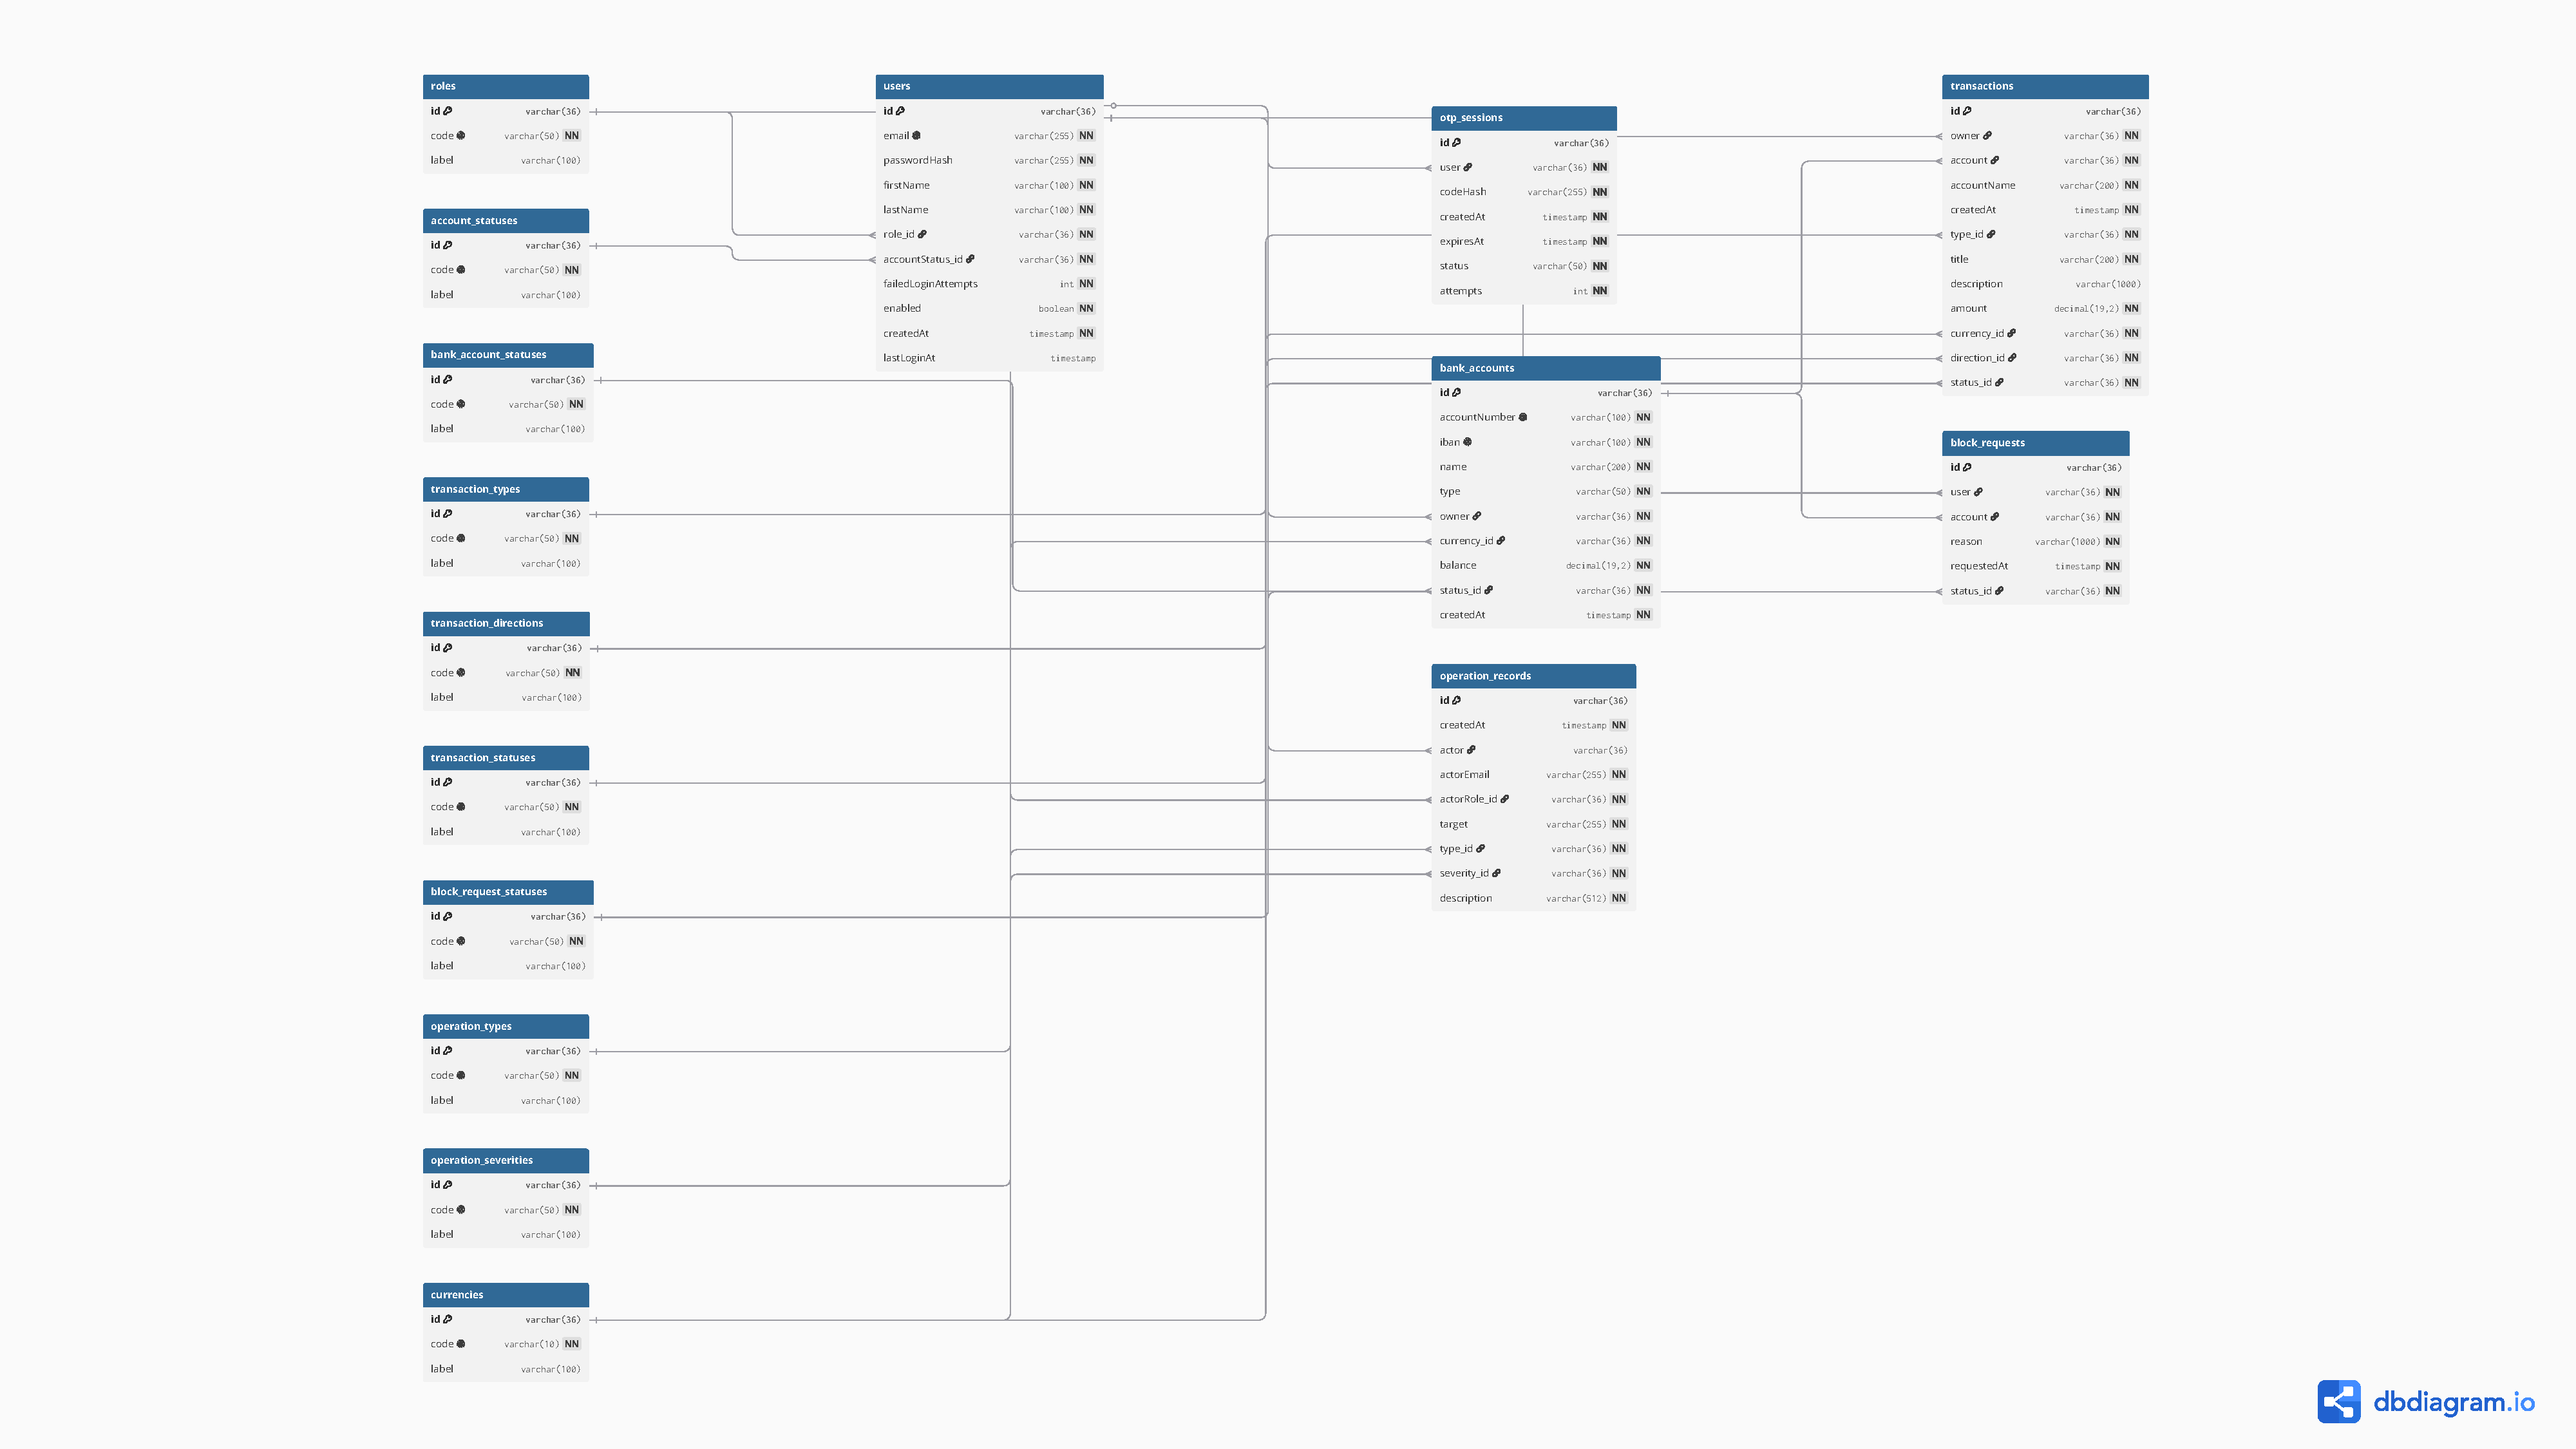
\includegraphics[width=\textwidth]{erd.pdf}
  \caption{Entity-Relationship Diagram — full schema with 16 tables and all
           foreign key relationships.}
  \label{fig:erd}
\end{figure}

\section{Schema Overview}

The schema consists of \textbf{16 tables} in three groups:

\begin{itemize}
  \item \textbf{6 core entity tables}: \texttt{users}, \texttt{bank\_accounts},
        \texttt{transactions}, \texttt{block\_requests}, \texttt{otp\_sessions},
        \texttt{operation\_records}.
  \item \textbf{10 lookup tables}: \texttt{roles}, \texttt{account\_statuses},
        \texttt{bank\_account\_statuses}, \texttt{transaction\_types},
        \texttt{transaction\_directions}, \texttt{transaction\_statuses},
        \texttt{block\_request\_statuses}, \texttt{operation\_types},
        \texttt{operation\_severities}, \texttt{currencies}.
\end{itemize}

All primary keys are UUIDs generated by the application (not database sequences),
which avoids exposing sequential identifiers to clients and makes distributed
generation possible in future.

\section{Core Entity Tables}

\subsection{users}

\begin{table}[H]
  \centering
  \caption{\texttt{users} table}
  \begin{tabular}{llll}
    \toprule
    \textbf{Column} & \textbf{Type} & \textbf{Constraints} & \textbf{Notes} \\
    \midrule
    id                    & varchar(36)  & PK              & UUID \\
    email                 & varchar(255) & UNIQUE, NOT NULL & Login identifier \\
    passwordHash          & varchar(255) & NOT NULL         & BCrypt hash \\
    firstName             & varchar(100) & NOT NULL         & \\
    lastName              & varchar(100) & NOT NULL         & \\
    role\_id              & varchar(36)  & FK → roles       & \\
    accountStatus\_id     & varchar(36)  & FK → account\_statuses & \\
    failedLoginAttempts   & int          & NOT NULL, default 0 & \\
    enabled               & boolean      & NOT NULL         & Spring Security flag \\
    createdAt             & timestamp    & NOT NULL         & \\
    lastLoginAt           & timestamp    & nullable         & Updated on OTP verify \\
    \bottomrule
  \end{tabular}
\end{table}

\subsection{bank\_accounts}

\begin{table}[H]
  \centering
  \caption{\texttt{bank\_accounts} table}
  \begin{tabular}{llll}
    \toprule
    \textbf{Column} & \textbf{Type} & \textbf{Constraints} & \textbf{Notes} \\
    \midrule
    id             & varchar(36)   & PK              & UUID \\
    accountNumber  & varchar(100)  & UNIQUE, NOT NULL & Internal number \\
    iban           & varchar(100)  & UNIQUE, NOT NULL & IBAN format \\
    name           & varchar(200)  & NOT NULL         & Display name \\
    type           & varchar(50)   & NOT NULL         & e.g. Current, Savings \\
    owner          & varchar(36)   & FK → users       & \\
    currency\_id   & varchar(36)   & FK → currencies  & \\
    balance        & decimal(19,2) & NOT NULL, default 0 & \\
    status\_id     & varchar(36)   & FK → bank\_account\_statuses & \\
    createdAt      & timestamp     & NOT NULL         & \\
    \bottomrule
  \end{tabular}
\end{table}

\subsection{transactions}

\begin{table}[H]
  \centering
  \caption{\texttt{transactions} table}
  \begin{tabular}{llll}
    \toprule
    \textbf{Column} & \textbf{Type} & \textbf{Constraints} & \textbf{Notes} \\
    \midrule
    id           & varchar(36)   & PK              & UUID \\
    owner        & varchar(36)   & FK → users      & Index: idx\_tx\_owner \\
    account      & varchar(36)   & FK → bank\_accounts & Index: idx\_tx\_account \\
    accountName  & varchar(200)  & NOT NULL        & Snapshot at time of TX \\
    createdAt    & timestamp     & NOT NULL        & Index: idx\_tx\_created \\
    type\_id     & varchar(36)   & FK → transaction\_types & \\
    title        & varchar(200)  & NOT NULL        & \\
    description  & varchar(1000) & nullable        & \\
    amount       & decimal(19,2) & NOT NULL        & Always positive \\
    currency\_id & varchar(36)   & FK → currencies & \\
    direction\_id& varchar(36)   & FK → transaction\_directions & DEBIT or CREDIT \\
    status\_id   & varchar(36)   & FK → transaction\_statuses & \\
    \bottomrule
  \end{tabular}
\end{table}

\subsection{block\_requests}

\begin{table}[H]
  \centering
  \caption{\texttt{block\_requests} table}
  \begin{tabular}{llll}
    \toprule
    \textbf{Column} & \textbf{Type} & \textbf{Constraints} & \textbf{Notes} \\
    \midrule
    id           & varchar(36)   & PK              & UUID \\
    user         & varchar(36)   & FK → users      & Who submitted the request \\
    account      & varchar(36)   & FK → bank\_accounts & Which account to block \\
    reason       & varchar(1000) & NOT NULL        & Customer's explanation \\
    requestedAt  & timestamp     & NOT NULL        & \\
    status\_id   & varchar(36)   & FK → block\_request\_statuses & \\
    \bottomrule
  \end{tabular}
\end{table}

\subsection{otp\_sessions}

\begin{table}[H]
  \centering
  \caption{\texttt{otp\_sessions} table}
  \begin{tabular}{llll}
    \toprule
    \textbf{Column} & \textbf{Type} & \textbf{Constraints} & \textbf{Notes} \\
    \midrule
    id         & varchar(36)  & PK              & UUID \\
    user       & varchar(36)  & FK → users      & \\
    codeHash   & varchar(255) & NOT NULL        & BCrypt hash of OTP code \\
    createdAt  & timestamp    & NOT NULL        & \\
    expiresAt  & timestamp    & NOT NULL        & now + 5 minutes \\
    status     & varchar(50)  & NOT NULL        & PENDING / USED / EXPIRED \\
    attempts   & int          & NOT NULL, default 0 & Blocks after 3 wrong tries \\
    \bottomrule
  \end{tabular}
\end{table}

\subsection{operation\_records}

\begin{table}[H]
  \centering
  \caption{\texttt{operation\_records} table (audit log)}
  \begin{tabular}{llll}
    \toprule
    \textbf{Column}  & \textbf{Type} & \textbf{Constraints} & \textbf{Notes} \\
    \midrule
    id           & varchar(36)  & PK                  & UUID \\
    createdAt    & timestamp    & NOT NULL            & Index \\
    actor        & varchar(36)  & FK → users, nullable & Null for system events \\
    actorEmail   & varchar(255) & NOT NULL            & Denormalised snapshot \\
    actorRole\_id& varchar(36)  & FK → roles          & Index \\
    target       & varchar(255) & NOT NULL            & Index \\
    type\_id     & varchar(36)  & FK → operation\_types & \\
    severity\_id & varchar(36)  & FK → operation\_severities & \\
    description  & varchar(512) & NOT NULL            & \\
    \bottomrule
  \end{tabular}
\end{table}

\section{Lookup Tables}

All ten lookup tables follow the same structure:

\begin{table}[H]
  \centering
  \caption{Lookup table structure (applied to all 10 domain tables)}
  \begin{tabular}{llll}
    \toprule
    \textbf{Column} & \textbf{Type} & \textbf{Constraints} & \textbf{Notes} \\
    \midrule
    id    & varchar(36)  & PK              & UUID \\
    code  & varchar(50)  & UNIQUE, NOT NULL & Matches Java enum name \\
    label & varchar(100) & nullable         & Human-readable description \\
    \bottomrule
  \end{tabular}
\end{table}

Table~\ref{tab:lookups} lists all ten lookup tables and their valid code values.

\begin{table}[H]
  \centering
  \caption{Lookup tables and their code values}
  \label{tab:lookups}
  \begin{tabular}{ll}
    \toprule
    \textbf{Table} & \textbf{Valid code values} \\
    \midrule
    roles                   & ADMIN, EMPLOYEE, CUSTOMER \\
    account\_statuses       & ACTIVE, LOCKED\_LOGIN\_FAILURE, BLOCKED\_BY\_BANK,
                              BLOCKED\_BY\_CUSTOMER\_REQUEST \\
    bank\_account\_statuses & ACTIVE, PENDING\_BLOCK, BLOCKED \\
    transaction\_types      & TRANSFER, PAYMENT, DEPOSIT \\
    transaction\_directions & DEBIT, CREDIT \\
    transaction\_statuses   & COMPLETED, PENDING, FAILED \\
    block\_request\_statuses& PENDING, APPROVED, REJECTED \\
    operation\_types        & LOGIN\_FAILURE, LOGIN\_SUCCESS, OTP\_VERIFIED,
                              TRANSFER\_CREATED, PAYMENT\_CREATED,
                              STATEMENT\_DOWNLOADED, HISTORY\_DOWNLOADED,
                              ACCOUNT\_BLOCK\_REQUESTED, ACCOUNT\_BLOCKED,
                              ACCOUNT\_UNBLOCKED, ACCESS\_UNBLOCKED,
                              CUSTOMER\_REGISTERED \\
    operation\_severities   & INFO, WARNING, CRITICAL, SUCCESS \\
    currencies              & EUR (and others as needed) \\
    \bottomrule
  \end{tabular}
\end{table}

\section{Entity Relationships}

Table~\ref{tab:rels} lists all foreign key relationships in the schema.

\begin{table}[H]
  \centering
  \caption{Entity relationships}
  \label{tab:rels}
  \begin{tabular}{lll}
    \toprule
    \textbf{From} & \textbf{To} & \textbf{Type} \\
    \midrule
    users                & roles                   & Many-to-One \\
    users                & account\_statuses        & Many-to-One \\
    bank\_accounts       & users                   & Many-to-One (owner) \\
    bank\_accounts       & bank\_account\_statuses  & Many-to-One \\
    bank\_accounts       & currencies              & Many-to-One \\
    transactions         & users                   & Many-to-One (owner) \\
    transactions         & bank\_accounts           & Many-to-One \\
    transactions         & transaction\_types       & Many-to-One \\
    transactions         & transaction\_directions  & Many-to-One \\
    transactions         & transaction\_statuses    & Many-to-One \\
    transactions         & currencies              & Many-to-One \\
    block\_requests      & users                   & Many-to-One \\
    block\_requests      & bank\_accounts           & Many-to-One \\
    block\_requests      & block\_request\_statuses & Many-to-One \\
    otp\_sessions        & users                   & Many-to-One \\
    operation\_records   & users (actor)           & Many-to-One (nullable) \\
    operation\_records   & roles                   & Many-to-One \\
    operation\_records   & operation\_types         & Many-to-One \\
    operation\_records   & operation\_severities    & Many-to-One \\
    \bottomrule
  \end{tabular}
\end{table}

\section{Key Design Decisions}

\textbf{UUID primary keys.} All tables use UUID primary keys generated by the
application layer (JPA \texttt{@GeneratedValue}). This avoids exposing predictable
sequential IDs to clients and is compatible with distributed generation.

\textbf{DECIMAL(19,2) for monetary values.} The \texttt{balance} and \texttt{amount}
columns use \texttt{DECIMAL(19,2)} (mapped to Java's \texttt{BigDecimal}) rather than
\texttt{FLOAT} or \texttt{DOUBLE}. Floating-point binary representation is inherently
imprecise for decimal fractions — for example, \texttt{0.1 + 0.2} in IEEE 754 double
precision is \texttt{0.30000000000000004}, not \texttt{0.30}. For a banking system,
this is unacceptable.

\textbf{BTREE indexes.} Three indexes are defined on \texttt{transactions}
(\texttt{owner}, \texttt{account}, \texttt{createdAt}) and three on
\texttt{operation\_records} (\texttt{actorEmail}, \texttt{target}, \texttt{createdAt}).
These cover the most frequent query patterns: loading a user's transaction list and
filtering the audit log by date.

\textbf{accountName snapshot in transactions.} The \texttt{accountName} column in
\texttt{transactions} stores the account name at the time of the transaction.
This is intentional denormalisation: if the account name changes later, the historical
transaction record still shows the correct name.

\textbf{actor nullable in operation\_records.} The \texttt{actor} FK in
\texttt{operation\_records} is nullable to allow system-generated events (e.g. the
automatic seeding of demo data) to be recorded without a specific user actor.
The \texttt{actorEmail} column stores a snapshot of the email regardless,
so the record is always identifiable.

% =========================================================
% CHAPTER 5 — BACKEND ARCHITECTURE
% =========================================================
\chapter{Backend Architecture}
\label{ch:backend}

\section{Package Structure}

The backend is a standard Spring Boot 3 application with the following package layout:


\textit{\small Backend package structure}\vspace{2pt}
\begin{Verbatim}[frame=single,fontsize=\small,bgcolor=codegray]
com.example.banking
|-- controller/     REST controllers (HTTP layer)
|-- service/        Business logic
|-- model/          JPA entities (16 tables)
|-- repository/     Spring Data JPA repositories
|-- security/       JWT filter, JWT service, SecurityConfig
`-- dto/            Request and response objects
\end{Verbatim}


\section{Security Filter Chain}

Every HTTP request passes through the \texttt{JwtAuthenticationFilter} before
reaching any controller. The filter performs the following steps:

\begin{enumerate}
  \item Extract the \texttt{Authorization: Bearer <token>} header.
  \item If no header is present, pass the request through (unauthenticated — Spring
        Security will enforce access rules downstream).
  \item Parse and validate the JWT signature and expiry using \texttt{JwtService}.
  \item Load the \texttt{User} entity from the database by the email claim.
  \item Check that \texttt{user.accountStatus} is \texttt{ACTIVE} — a locked or
        blocked user is rejected even with a valid token.
  \item Set a \texttt{UsernamePasswordAuthenticationToken} in the
        \texttt{SecurityContextHolder} with the user and their role.
\end{enumerate}


\textit{\small Core JWT validation logic in JwtAuthenticationFilter}\vspace{2pt}
\begin{Verbatim}[frame=single,fontsize=\small,bgcolor=codegray]
User user = userRepository.findByEmail(email).orElse(null);
if (user == null || !user.getAccountStatus().is(AccountStatus.ACTIVE)) {
    response.sendError(SC_UNAUTHORIZED, "User not found or access blocked");
    return;
}
UsernamePasswordAuthenticationToken auth =
    new UsernamePasswordAuthenticationToken(
        user, null,
        List.of(new SimpleGrantedAuthority("ROLE_" + user.getRole().getCode()))
    );
SecurityContextHolder.getContext().setAuthentication(auth);
filterChain.doFilter(request, response);
\end{Verbatim}


\section{JWT Implementation}

Tokens are generated by \texttt{JwtService} using the JJWT library with HMAC-SHA256
signing. Each token contains:

\begin{itemize}[noitemsep]
  \item \textbf{Subject}: user email address.
  \item \textbf{role claim}: the user's role code (e.g. \texttt{"CUSTOMER"}).
  \item \textbf{userId claim}: the user's UUID.
  \item \textbf{Issued at}: current instant.
  \item \textbf{Expiry}: issued-at plus one hour.
\end{itemize}

The signing secret is provided via the \texttt{APP\_JWT\_SECRET} environment variable
and must be at least 32 characters long for HMAC-SHA256.

\section{Two-Factor Authentication Flow}

Login is a two-step process. A JWT is only issued after both steps succeed.

\textbf{Step 1 — Password verification} (\texttt{POST /api/auth/login}):
\begin{enumerate}[noitemsep]
  \item Look up the user by email.
  \item Check \texttt{accountStatus} is ACTIVE.
  \item Verify password against the BCrypt hash.
  \item If wrong: increment \texttt{failedLoginAttempts}; if now $\geq 3$, set status
        to \texttt{LOCKED\_LOGIN\_FAILURE} and record a CRITICAL audit event.
  \item If correct: reset \texttt{failedLoginAttempts} to 0; generate a 6-digit OTP;
        store its BCrypt hash in a new \texttt{OtpSession} (expires in 5 minutes,
        status PENDING); return the \texttt{otpSessionId}.
\end{enumerate}

\textbf{Step 2 — OTP verification} (\texttt{POST /api/auth/verify-otp}):
\begin{enumerate}[noitemsep]
  \item Find \texttt{OtpSession} by ID where status = PENDING.
  \item Check \texttt{expiresAt} has not passed.
  \item Verify the submitted code against \texttt{codeHash} using BCrypt.
  \item If wrong: increment \texttt{attempts}; if $\geq 3$, set status to EXPIRED.
  \item If correct: set status to USED; update \texttt{user.lastLoginAt}; issue JWT.
\end{enumerate}

\section{Service Layer}

\begin{table}[H]
  \centering
  \caption{Core service classes and their responsibilities}
  \begin{tabular}{lp{9cm}}
    \toprule
    \textbf{Service} & \textbf{Responsibility} \\
    \midrule
    AuthService       & Registration, login (2FA), OTP verification. \\
    CustomerService   & Account overview, transfers, payments, block requests,
                        CSV downloads. \\
    AdminService      & Dashboard statistics, customer listing, security queue,
                        account block/unblock, block request approval/rejection,
                        user unlock. \\
    OperationService  & Records all audit events into \texttt{operation\_records}. \\
    BootstrapService  & Seeds lookup tables (idempotently) and demo data on startup. \\
    \bottomrule
  \end{tabular}
\end{table}

\section{Exception Handling}

\texttt{GlobalExceptionHandler} catches all exceptions thrown from services and maps
them to appropriate HTTP status codes:

\begin{table}[H]
  \centering
  \caption{Exception to HTTP status mapping}
  \begin{tabular}{ll}
    \toprule
    \textbf{Exception} & \textbf{HTTP Status} \\
    \midrule
    IllegalArgumentException          & 400 Bad Request \\
    MethodArgumentNotValidException   & 400 Bad Request \\
    EntityNotFoundException           & 404 Not Found \\
    IllegalStateException             & 423 Locked \\
    AccessDeniedException             & 403 Forbidden \\
    Exception (fallback)              & 500 Internal Server Error \\
    \bottomrule
  \end{tabular}
\end{table}

All error responses follow a standard JSON envelope:


\textit{\small Standard error response format}\vspace{2pt}
\begin{Verbatim}[frame=single,fontsize=\small,bgcolor=codegray]
{
  "timestamp": "2026-06-10T20:00:00Z",
  "status": 400,
  "error": "Bad Request",
  "message": "Insufficient balance",
  "path": "/api/customer/transfers"
}
\end{Verbatim}


% =========================================================
% CHAPTER 6 — FRONTEND ARCHITECTURE
% =========================================================
\chapter{Frontend Architecture}
\label{ch:frontend}

\section{Overview}

The frontend is a React 18 single-page application written in TypeScript, built with
Vite, and using Ant Design for UI components. In production, the compiled static bundle
is served by Nginx inside a Docker container.

\section{Routing}

React Router v6 is used for client-side routing. Routes are divided into three groups:

\begin{itemize}
  \item \textbf{Public routes}: \texttt{/}, \texttt{/login}, \texttt{/register},
        \texttt{/verify-otp}.
  \item \textbf{Customer routes}: \texttt{/customer/overview}, \texttt{/customer/accounts},
        \texttt{/customer/payments}, \texttt{/customer/activity}.
  \item \textbf{Admin routes}: \texttt{/admin/overview}, \texttt{/admin/customers},
        \texttt{/admin/operations}, \texttt{/admin/security}.
\end{itemize}

\texttt{ProtectedRoute} is a wrapper component that reads the JWT from
\texttt{localStorage}, checks the user's role, and redirects to the login page if
the user is unauthenticated or to their role's home page if they attempt to access
a route outside their role.

\section{Authentication Context}

\texttt{AuthProvider} is a React context that wraps the entire application and exposes:

\begin{itemize}[noitemsep]
  \item \texttt{user} — the current \texttt{UserDto} loaded from \texttt{localStorage}.
  \item \texttt{token} — the JWT string stored in \texttt{localStorage}.
  \item \texttt{login()} — submits credentials, stores the \texttt{otpSessionId} in
        \texttt{sessionStorage}.
  \item \texttt{verifyOtp()} — submits the OTP, receives the JWT and stores it in
        \texttt{localStorage}.
  \item \texttt{logout()} — clears all storage and resets context state.
\end{itemize}

\section{API Client}

All HTTP requests go through a shared \texttt{api/client.ts} module that:
\begin{itemize}[noitemsep]
  \item Reads the JWT from \texttt{localStorage} automatically.
  \item Injects \texttt{Authorization: Bearer <token>} on every request.
  \item Sets \texttt{Content-Type: application/json} for request bodies.
  \item Throws a typed error if \texttt{response.ok} is false, including the HTTP
        status and server error message.
\end{itemize}

% =========================================================
% CHAPTER 7 — API DESIGN
% =========================================================
\chapter{API Design}
\label{ch:api}

\section{Endpoint Overview}

\begin{table}[H]
  \centering
  \caption{REST API endpoints}
  \label{tab:api}
  \begin{tabular}{lllp{5cm}}
    \toprule
    \textbf{Method} & \textbf{Path} & \textbf{Role} & \textbf{Description} \\
    \midrule
    POST & /api/auth/register           & Public   & Register new customer \\
    POST & /api/auth/login              & Public   & Step 1: password check \\
    POST & /api/auth/verify-otp         & Public   & Step 2: OTP check + JWT \\
    GET  & /api/me                      & Any      & Current user profile \\
    GET  & /api/health                  & Public   & Health check \\
    \midrule
    GET  & /api/customer/overview       & CUSTOMER & Dashboard data \\
    GET  & /api/customer/accounts       & CUSTOMER & Account list \\
    GET  & /api/customer/activity       & CUSTOMER & Transaction history \\
    POST & /api/customer/transfers      & CUSTOMER & Create transfer \\
    POST & /api/customer/payments       & CUSTOMER & Create payment \\
    POST & /api/customer/accounts/\{id\}/request-block & CUSTOMER & Request block \\
    GET  & /api/customer/downloads/statement & CUSTOMER & CSV statement \\
    GET  & /api/customer/downloads/history   & CUSTOMER & CSV history \\
    \midrule
    GET  & /api/admin/dashboard         & ADMIN    & System statistics \\
    GET  & /api/admin/customers         & ADMIN    & Customer list \\
    GET  & /api/admin/operations        & ADMIN    & Full audit log \\
    GET  & /api/admin/security          & ADMIN    & Security queue \\
    POST & /api/admin/users/\{id\}/unlock-access     & ADMIN & Unlock user \\
    POST & /api/admin/accounts/\{id\}/block          & ADMIN & Block account \\
    POST & /api/admin/accounts/\{id\}/unblock        & ADMIN & Unblock account \\
    POST & /api/admin/block-requests/\{id\}/approve  & ADMIN & Approve request \\
    POST & /api/admin/block-requests/\{id\}/reject   & ADMIN & Reject request \\
    \bottomrule
  \end{tabular}
\end{table}

\section{HTTP Status Codes}

\begin{table}[H]
  \centering
  \caption{HTTP status codes used by the API}
  \begin{tabular}{ll}
    \toprule
    \textbf{Code} & \textbf{Meaning} \\
    \midrule
    200 & Success \\
    201 & Resource created (registration) \\
    400 & Validation error, wrong password, insufficient balance \\
    401 & Missing or invalid JWT token \\
    403 & Insufficient role \\
    404 & Resource not found \\
    423 & Account or user is locked / blocked \\
    500 & Internal server error \\
    \bottomrule
  \end{tabular}
\end{table}

% =========================================================
% CHAPTER 8 — SECURITY MODEL
% =========================================================
\chapter{Security Model}
\label{ch:security}

\section{Two-Factor Authentication}

As described in Chapter~\ref{ch:backend}, login requires both a correct password
and a valid OTP. The OTP is a 6-digit numeric code that expires after five minutes.
In this prototype, the OTP is written to the application log (prefixed with
\texttt{[DEV]}). A production system would replace this with an email or SMS delivery.

The OTP code is never stored in plaintext — it is hashed with BCrypt before being
written to the database. Verification uses \texttt{passwordEncoder.matches()},
the same mechanism used for password verification.

\section{Account Locking}

After three consecutive incorrect password entries, the user's \texttt{accountStatus}
is set to \texttt{LOCKED\_LOGIN\_FAILURE}. The account is then rejected at two points:
\begin{itemize}[noitemsep]
  \item During login (before OTP generation).
  \item During every subsequent request (in \texttt{JwtAuthenticationFilter}, even
        with a valid token).
\end{itemize}

An administrator must explicitly call \texttt{POST /api/admin/users/\{id\}/unlock-access}
to restore access. This resets \texttt{accountStatus} to \texttt{ACTIVE} and sets
\texttt{failedLoginAttempts} to 0.

\section{Account Blocking Workflow}

Bank accounts (not user logins) can be blocked through two paths:

\textbf{Customer-initiated:}
\begin{enumerate}[noitemsep]
  \item Customer submits a block request with a reason.
  \item Account status changes to \texttt{PENDING\_BLOCK}.
  \item Admin approves → account status becomes \texttt{BLOCKED}.
  \item Admin rejects → account status reverts to \texttt{ACTIVE}.
\end{enumerate}

\textbf{Admin-initiated:}
\begin{enumerate}[noitemsep]
  \item Admin calls the block endpoint directly.
  \item Account status immediately becomes \texttt{BLOCKED}.
  \item Any pending block request for that account is auto-approved.
\end{enumerate}

\textbf{Effect of blocking:} Transfers and payments from a \texttt{BLOCKED} or
\texttt{PENDING\_BLOCK} account throw an exception before any balance mutation.

\section{Audit Logging}

Every security-relevant action produces a row in \texttt{operation\_records} via
\texttt{OperationService.record()}. Table~\ref{tab:audit} shows the severity levels.

\begin{table}[H]
  \centering
  \caption{Audit log severity levels and example events}
  \label{tab:audit}
  \begin{tabular}{lll}
    \toprule
    \textbf{Severity} & \textbf{Example events} \\
    \midrule
    INFO     & Login success, OTP verified, transfer created, history downloaded \\
    WARNING  & Failed login attempt, account block requested \\
    CRITICAL & Account blocked after 3 login failures, account blocked by admin \\
    SUCCESS  & User access restored, account unblocked \\
    \bottomrule
  \end{tabular}
\end{table}

\section{Known Limitations}

\begin{table}[H]
  \centering
  \caption{Known security limitations}
  \begin{tabular}{lp{9cm}}
    \toprule
    \textbf{Area} & \textbf{Limitation} \\
    \midrule
    OTP delivery   & OTP is only logged to console. No email/SMS delivery. \\
    Race conditions& No optimistic locking (\texttt{@Version}) on balance updates.
                     Two concurrent transfers from the same account could both pass
                     the balance check. \\
    Token revocation & Issued JWTs cannot be invalidated before expiry. \\
    Rate limiting  & No rate limiting on login or OTP endpoints. \\
    \bottomrule
  \end{tabular}
\end{table}

% =========================================================
% CHAPTER 9 — TESTING
% =========================================================
\chapter{Testing}
\label{ch:testing}

\section{Test Strategy}

The project uses three levels of testing:
\begin{itemize}[noitemsep]
  \item \textbf{Unit tests}: test individual service classes with all dependencies
        mocked using Mockito.
  \item \textbf{Integration tests}: start the full Spring Boot context with an H2
        in-memory database and test HTTP endpoints via MockMvc.
  \item \textbf{End-to-end tests}: Playwright scripts run against the live Docker
        Compose stack and simulate real user interactions in a browser.
\end{itemize}

Run all backend tests with:

\textit{\small Running backend tests}\vspace{2pt}
\begin{Verbatim}[frame=single,fontsize=\small,bgcolor=codegray]
docker run --rm \
  -v "$(pwd)/backend:/app" \
  -v "$HOME/.m2:/root/.m2" \
  -w /app maven:3.9.8-eclipse-temurin-21 \
  mvn test
\end{Verbatim}


\section{Unit Tests}

\begin{table}[H]
  \centering
  \caption{Unit test classes and scenario counts}
  \begin{tabular}{lll}
    \toprule
    \textbf{Class} & \textbf{Scenarios} & \textbf{What is verified} \\
    \midrule
    JwtServiceTest       & 5 & Token generation, subject/role extraction,
                               tamper detection, empty string \\
    AuthServiceTest      & 9 & Registration, login failures, locking,
                               OTP expiry, wrong code, success flow \\
    CustomerServiceTest  & 8 & Transfer validation, internal double-booking,
                               payment, block request \\
    AdminServiceTest     & 7 & Unlock user, block/unblock account,
                               approve/reject block request \\
    \bottomrule
  \end{tabular}
\end{table}

\section{Integration Tests}

\begin{table}[H]
  \centering
  \caption{Integration test classes}
  \begin{tabular}{lll}
    \toprule
    \textbf{Class} & \textbf{Tests} & \textbf{What is verified} \\
    \midrule
    AuthIntegrationTest     & 5 & Register 201, unknown email 404,
                                  wrong password 400, locked 423,
                                  invalid OTP session 404 \\
    CustomerIntegrationTest & 3 & 401 without token, 403 for admin role \\
    AdminIntegrationTest    & 3 & 401 without token, 403 for customer role \\
    SecurityIntegrationTest & 5 & Health public, protected 401, cross-role 403 \\
    \bottomrule
  \end{tabular}
\end{table}

\section{Test Results}

All 46 tests pass on every build:


\textit{\small Maven test output}\vspace{2pt}
\begin{Verbatim}[frame=single,fontsize=\small,bgcolor=codegray]
Tests run: 46, Failures: 0, Errors: 0, Skipped: 0
BUILD SUCCESS
Total time: 29.845 s
\end{Verbatim}


\section{Coverage Gaps}

\begin{table}[H]
  \centering
  \caption{Known test coverage gaps}
  \begin{tabular}{lp{9cm}}
    \toprule
    \textbf{Area} & \textbf{Gap} \\
    \midrule
    OTP delivery        & No test for email/SMS delivery (console-only in prototype). \\
    CSV downloads       & \texttt{downloadStatement()} and \texttt{downloadHistory()}
                          not directly tested. \\
    Concurrent TX       & No test for race condition on simultaneous transfers. \\
    Frontend unit tests & No React component unit tests (Vitest / RTL). \\
    Full E2E flow       & Playwright suite covers happy paths only; no negative
                          scenario automation. \\
    \bottomrule
  \end{tabular}
\end{table}

% =========================================================
% CHAPTER 10 — APPLICATION WALKTHROUGH
% =========================================================
\chapter{Application Walkthrough}
\label{ch:walkthrough}

This chapter provides a visual walkthrough of the application using screenshots taken
from a live demo session. All screenshots are taken from the running Docker Compose
stack.

\section{Landing Page}

\begin{figure}[H]
  \centering
  \includegraphics[width=0.9\textwidth]{01-landing-page-hero.png}
  \caption{Landing page — hero section. The public homepage presents the platform
           concept and provides navigation to login and register.}
  \label{fig:landing-hero}
\end{figure}

\begin{figure}[H]
  \centering
  \includegraphics[width=0.9\textwidth]{02-landing-page-roles.png}
  \caption{Landing page — roles section. Describes the two primary roles (Customer
           and Administrator) and offers quick access to the login modal with pre-filled
           demo credentials.}
  \label{fig:landing-roles}
\end{figure}

\section{Login and Two-Factor Authentication}

\begin{figure}[H]
  \centering
  \includegraphics[width=0.9\textwidth]{09-login-modal-customer.png}
  \caption{Login modal — step 1. The user enters their email and password. Demo
           credential shortcuts are provided for each role.}
  \label{fig:login-modal}
\end{figure}

\begin{figure}[H]
  \centering
  \includegraphics[width=0.9\textwidth]{03-login-otp-verification.png}
  \caption{OTP verification modal — step 2. After a successful password check, the
           user must enter the 6-digit OTP code retrieved from the backend log
           (\texttt{[DEV] OTP for admin@bank.local: 022006}).}
  \label{fig:otp}
\end{figure}

\section{Admin Dashboard}

\begin{figure}[H]
  \centering
  \includegraphics[width=0.9\textwidth]{04-admin-overview-stats.png}
  \caption{Admin overview — system statistics. Shows total customers (3), total funds
           across all accounts (\euro{}26,855.58), blocked users (1), and pending block
           requests (1).}
  \label{fig:admin-stats}
\end{figure}

\begin{figure}[H]
  \centering
  \includegraphics[width=0.9\textwidth]{05-admin-overview-recent-events.png}
  \caption{Admin overview — recent high-priority events. The dashboard shows the latest
           CRITICAL and WARNING events from the audit log, including the locked customer
           incident and Brian's block request.}
  \label{fig:admin-events}
\end{figure}

\begin{figure}[H]
  \centering
  \includegraphics[width=0.9\textwidth]{06-admin-security-queue.png}
  \caption{Admin security queue. Three sections: pending block requests (Brian Walsh's
           request with Approve/Reject buttons), blocked access users (Locked Customer
           with Restore access), and blocked accounts (empty at this point).}
  \label{fig:admin-security}
\end{figure}

\begin{figure}[H]
  \centering
  \includegraphics[width=0.9\textwidth]{07-admin-operations-audit-log.png}
  \caption{Admin operations — full audit log. Every action is recorded: account
           unblock, account block, access restore, login success, login failure,
           block request, and payment. Searchable and filterable by severity and type.}
  \label{fig:admin-log}
\end{figure}

\begin{figure}[H]
  \centering
  \includegraphics[width=0.9\textwidth]{08-admin-customer-administration.png}
  \caption{Admin customer administration. Lists all customers with access status,
           failed attempts, account counts, pending requests, and last login.
           A ``Manage'' action opens a customer detail drawer.}
  \label{fig:admin-customers}
\end{figure}

\section{Customer Dashboard}

\begin{figure}[H]
  \centering
  \includegraphics[width=0.9\textwidth]{10-customer-overview-dashboard.png}
  \caption{Customer overview — Alice Murphy's dashboard. Shows total balance
           (\euro{}24,665.18), 2 active accounts, and the 5 most recent transactions
           with types, statuses, and amounts.}
  \label{fig:customer-overview}
\end{figure}

\begin{figure}[H]
  \centering
  \includegraphics[width=0.9\textwidth]{11-customer-accounts.png}
  \caption{Customer accounts page. Shows both accounts with IBAN, account number,
           currency, balance, and status. The detail panel provides download and block
           request actions.}
  \label{fig:customer-accounts}
\end{figure}

\begin{figure}[H]
  \centering
  \includegraphics[width=0.9\textwidth]{12-customer-payments-transfers.png}
  \caption{Payments and transfers page. The Transfer tab allows sending funds to an
           account number. The Bill Payment tab handles external payees. Only ACTIVE
           accounts are shown in the source account selector.}
  \label{fig:customer-payments}
\end{figure}

\begin{figure}[H]
  \centering
  \includegraphics[width=0.9\textwidth]{13-customer-transaction-history.png}
  \caption{Transaction history page. Shows all transactions with date, account, type,
           title, counterparty, status, and signed amount. Filterable by account and
           transaction type, with a CSV download option.}
  \label{fig:customer-history}
\end{figure}

% =========================================================
% CHAPTER 11 — DEPLOYMENT
% =========================================================
\chapter{Deployment}
\label{ch:deployment}

\section{Docker Compose Setup}

The entire system is defined in a single \texttt{docker-compose.yml} at the repository
root. Three services are configured:

\begin{table}[H]
  \centering
  \caption{Docker Compose services}
  \begin{tabular}{llll}
    \toprule
    \textbf{Service} & \textbf{Image} & \textbf{Port} & \textbf{Role} \\
    \midrule
    ib-db       & postgres:16                       & 5432 & PostgreSQL database \\
    ib-backend  & Multi-stage Maven + JRE build     & 8080 & Spring Boot API \\
    ib-frontend & Multi-stage Node.js + Nginx build & 5173 & React SPA \\
    \bottomrule
  \end{tabular}
\end{table}

\section{Environment Variables}

\begin{table}[H]
  \centering
  \caption{Key environment variables}
  \begin{tabular}{lll}
    \toprule
    \textbf{Variable} & \textbf{Default} & \textbf{Purpose} \\
    \midrule
    SPRING\_DATASOURCE\_URL      & jdbc:postgresql://db:5432/internet\_banking & DB connection \\
    SPRING\_DATASOURCE\_USERNAME & bank\_user  & DB username \\
    SPRING\_DATASOURCE\_PASSWORD & bank\_pass  & DB password \\
    APP\_JWT\_SECRET             & (change me) & JWT signing key \\
    APP\_ADMIN\_EMAIL            & admin@bank.local & Admin account email \\
    APP\_ADMIN\_PASSWORD         & Admin123!   & Admin account password \\
    APP\_SEED\_DEMO\_DATA        & true        & Seed demo users/data \\
    \bottomrule
  \end{tabular}
\end{table}

\section{Starting the Application}


\textit{\small Full startup sequence}\vspace{2pt}
\begin{Verbatim}[frame=single,fontsize=\small,bgcolor=codegray]
# Clone the repository
git clone <repo-url>
cd internet-banking-system

# Start all services (builds images if not cached)
docker compose up --build

# Access the application
# Frontend:  http://localhost:5173
# Backend:   http://localhost:8080
# Health:    http://localhost:8080/api/health

# Get OTP code during login
docker compose logs -f backend | grep "OTP for"

# Stop and remove all containers and volumes (clean reset)
docker compose down -v
\end{Verbatim}


% =========================================================
% CHAPTER 12 — CONCLUSIONS
% =========================================================
\chapter{Conclusions}
\label{ch:conclusions}

\section{Summary}

The Internet Banking System successfully demonstrates the design and implementation of a
secure, role-based web banking application. The key outcomes of the project are:

\begin{itemize}
  \item A fully functional three-tier web application deployable with a single command.
  \item A normalised relational database schema with 16 tables, lookup tables for all
        enumerated domains, and proper indexing.
  \item Two-factor authentication using BCrypt-hashed OTP codes.
  \item Role-based access control enforced at both the HTTP and business logic layers.
  \item Complete audit logging for all security-relevant actions.
  \item A comprehensive test suite with 46 passing tests across unit, integration,
        and end-to-end levels.
\end{itemize}

\section{Lessons Learned}

\textbf{Enum-as-table pattern.} The refactoring from plain VARCHAR enums to lookup
tables significantly increased the complexity of the application code (each enum
comparison now requires a database lookup or a helper method call), but the benefit
is a self-documenting, database-enforced domain model. For a system where domain values
rarely change, the VARCHAR approach is simpler; for a system that needs to support
configuration of valid values at runtime, lookup tables are the correct choice.

\textbf{Schema migration tooling.} Using \texttt{ddl-auto: update} in Hibernate is
convenient for development but caused issues when switching from the old schema (with
VARCHAR enums) to the new schema (with FK columns). In a production system, a proper
migration tool (Flyway or Liquibase) would manage schema changes safely without
requiring a full database wipe.

\textbf{BigDecimal for money.} The use of \texttt{DECIMAL(19,2)} and Java's
\texttt{BigDecimal} for all monetary values was essential. Float/double would introduce
rounding errors in financial calculations.

\section{Potential Improvements}

\begin{itemize}[noitemsep]
  \item \textbf{OTP delivery}: integrate a real email or SMS provider.
  \item \textbf{Optimistic locking}: add \texttt{@Version} to \texttt{BankAccount}
        to prevent race conditions on concurrent transfers.
  \item \textbf{Token revocation}: implement a token blacklist or use short-lived
        refresh tokens to allow logout to be enforced server-side.
  \item \textbf{Rate limiting}: add rate limiting on authentication endpoints to
        slow brute-force attacks beyond the 3-strike lock.
  \item \textbf{Schema migrations}: replace \texttt{ddl-auto: update} with Flyway
        for controlled, versioned schema changes.
  \item \textbf{Pagination}: add cursor-based pagination to transaction history
        and audit log endpoints for large datasets.
\end{itemize}

% =========================================================
% REFERENCES
% =========================================================
\chapter*{References}
\addcontentsline{toc}{chapter}{References}

\begin{enumerate}
  \item Spring Boot Documentation. \textit{Spring Boot Reference Guide 3.3}.
        Pivotal Software, 2024. \url{https://docs.spring.io/spring-boot/docs/3.3.x/reference/html/}

  \item Spring Security Documentation. \textit{Spring Security Reference 6.x}.
        Pivotal Software, 2024. \url{https://docs.spring.io/spring-security/reference/}

  \item JJWT Library. \textit{Java JWT: JSON Web Token for Java and Android}.
        Stormpath / jwtk, 2024. \url{https://github.com/jwtk/jjwt}

  \item React Documentation. \textit{React 18 — The Library for Web and Native User Interfaces}.
        Meta, 2024. \url{https://react.dev/}

  \item Ant Design. \textit{Ant Design 5.x Component Library}.
        Ant Group, 2024. \url{https://ant.design/}

  \item PostgreSQL Documentation. \textit{PostgreSQL 16 Documentation}.
        The PostgreSQL Global Development Group, 2024. \url{https://www.postgresql.org/docs/16/}

  \item Hibernate ORM. \textit{Hibernate ORM 6.5 User Guide}.
        Red Hat, 2024. \url{https://docs.jboss.org/hibernate/orm/6.5/userguide/html_single/}

  \item Docker Documentation. \textit{Docker Compose Reference}.
        Docker Inc., 2024. \url{https://docs.docker.com/compose/}

  \item Fowler, M. \textit{Patterns of Enterprise Application Architecture}.
        Addison-Wesley, 2002.

  \item OWASP. \textit{OWASP Top Ten — Web Application Security Risks}.
        OWASP Foundation, 2023. \url{https://owasp.org/www-project-top-ten/}
\end{enumerate}

\end{document}
